\refstepcounter{sdel}
\section{Scientific Deliverable \thesdel\ -- What is a Microservice?}
\label{sd:ms}

% {\color{gray}
% For each scientific deliverable targeted in section~\ref{sec-deliverables} provide a full section with all the subsections described below.
% \label{sec-production}
% }

\subsection{Requirements}% (± 15\% of section's words)}
% {\color{gray}
% Describe here all the properties that characterize the deliverables you produced. It should describe, for each main deliverable, what are the expected functional and non functional properties of the deliverables, who are the actors exploiting the deliverables. It is expected that you have at least one scientific deliverable (e.g. ``Scientific presentation of the Python programming language'', ``State of the art on quality models for human computer interaction'', \ldots.) and one technical deliverable (e.g. ``BSProSoft - A python/django web-site for IT job offers retrieval and analysis'', \ldots). 
% }

Since \glspl{ms} were a previously unknown concept to us, this
scientific deliverable targets the analysis of this architectural
style. In the design section we will briefly present our sources.  In
the production we will elaborate on motivations behind the
architecture and then explore what constitutes a \gls{ms}. The
assessment will highlight a few drawbacks of the \gls{ms}
architecture.

\subsection{Design}% (± 30\% of section's words)}
% {\color{gray}
% Provide the necessary and most useful explanations on how those deliverables have been produced.
% }

To conduct the research we mostly relied on articles and papers on the
matter. Articles \enquote{Microservices: A definition of this new architectural
term} \cite{ms-definition} and \enquote{Microservice Trade-Offs --
Operational Complexity (Con)} \cite{ms-trade-off} talked about
\glspl{ms} and allowed us to get a broad overview at this
architectural style.

The articles \enquote{DeploymentPipeline} \cite{pipelines} and
\enquote{devops-culture} \cite{devops-culture} delved into the DevOps
side of things. These also allowed us to get a clearer picture of how
both concepts of \gls{ms} and DevOps come together.

The remaining papers were then used to dig further into the matter and
to gather more insights in the \gls{ms} architecture and some of its
technical aspects. These insights were for the most part presented
through opinions of \gls{ms} practitioners which were collected
through surveys or observations. These papers include 
\enquote{A Survey on the Interplay between Software Engineering and Systems Engineering during SoS Architecting}
\cite{sos-survey},
\enquote{Challenges in Docker Development: A Large-scale Study Using Stack Overflow}
\cite{docker-so},
\enquote{Architecting with microservices: A systematic mapping study}
\cite{ms-arch-study},
\enquote{Challenges of production microservices}
\cite{ms-challenges},
\enquote{The pains and gains of microservices: A Systematic grey literature review}
\cite{ms-pains-gains} and
\enquote{Processes, Motivations, and Issues for Migrating to Microservices Architectures: An Empirical Investigation}
\cite{ms-migration}.

All the references have been provided by the \gls{bsp} tutor and have
been parsed for interesting information and insights to be presented
here. A separate document from this report was used to collect
everything. The foremost goal was to gather information that would
allow a reader to understand the \gls{ms} architecture. Then we delved
deeper into potential shortcomings and benefits, thus giving us a
better idea of how this architectural style is perceived by its
practitioners.

\subsection{Production}% (± 40\% of section's words)}
% {\color{gray}
% Provide descriptions of the deliverables concrete production. It must present part of the deliverable (e.g. source code extracts, scientific work extracts, \ldots) to illustrate and explain its actual production.
% }

A first simple definition can be found in the MSs article
\cite{ms-definition} that lays out some aspects which characterize a
MS architecture.

\begin{quote}
	In short, the microservice architectural style is an approach to
	developing a single application as a suite of small services,
	each running in its own process and communicating with lightweight
	mechanisms [\ldots]. These services are built around business
	capabilities and independently deployable by fully automated
	deployment machinery.  There
	is a bare minimum of centralized management of these services, which
	may be written in different programming languages and use different
	data storage technologies. 
\end{quote}

However, as stated multiple times in the article \cite{ms-definition},
there is no formal definition for MS. As such, we shall inspect
characteristics that such architectures tend to have in common a bit
later into this section.

To understand the benefits and motivations behind using \gls{ms} over
the monolithic style, we will first look at the latter.
\cite{ms-definition}

Monolithic architectures build applications using a single unit. This
basically means that all of an application's functionality, logic,
classes, function and name spaces are in the end located within a
single executable and thus run within a single process.
\cite{ms-definition} This model is very much usable in fact and allows
us to create functioning systems---as has demonstrated the time of
software development before \glspl{ms} were introduced. However, this
architectural style raises some issues nonetheless. For instance, even
the smallest of changes in an application require the whole product to
be rebuilt and redeployed or redistributed which is not necessarily
ideal in the case of large applications with multiple end-users.

As the application's life cycles goes on, it is unavoidable to modify
it over time. In a monolithic system however, it becomes increasingly
difficult to maintain a modular structure---if one was present to
begin with---which in turn also leads to modifications becoming more
expensive. \cite{ms-definition} The expensive modifications are
explained by the fact that if a modular structure cannot be
guaranteed, it possibly entails that changes to one component may
impact other components which were not supposed to be affected.
\cite{ms-definition} This may result in many adjacent changes and
unexpected issues to be performed and treated respectively.

Lastly, if we want to scale an application we actually need to scale
the application as a whole rather than the individual components that
need to be scaled.

\begin{figure*}
	\centering
	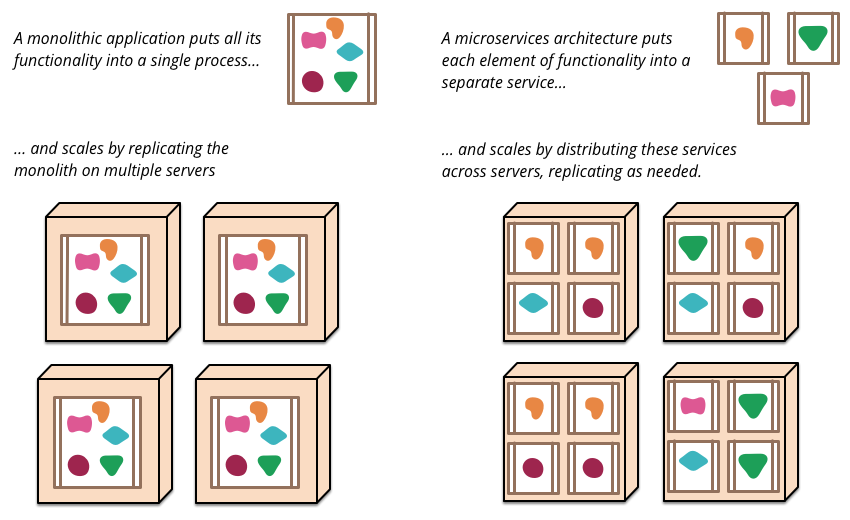
\includegraphics[width=0.75\linewidth]{images/sketch.png}
	\caption{Monoliths and Microservices \cite{ms-definition}}
	\label{fig:monoliths-ms}
\end{figure*}

Figure \ref{fig:monoliths-ms} nicely demonstrates some of the
aforementioned issues and how the \gls{ms} architecture tries to
tackle them.

Since the application is now split into separate services, making
modifications will not require us to build and deploy the whole
application anew. It will be enough to only update the services in
question.

Further, the fact that the application is built in a modular fashion
from the ground up and divided into smaller chunks and services makes
it easier to maintain a modular structure within the application as a
whole. As a result, making changes to one such service will guarantee
that none of the other services will be affected and thus keep
undesired or unforeseen side effects to a minimum.

We can also see that scaling an application becomes much less of a
burden. No longer do we need to scale the whole application, but we
can simply introduce new services where needed.

Moving on to the characteristics of \glspl{ms}.

\subsubsection{Componentization via Services}
\label{sec:componentization}

The article \cite{ms-definition} distinguishes between two types of
components---where \textit{component} refers to a unit of software
that is independently replaceable and upgradeable:

\begin{description}
	\item[libraries] which are being linked into a program and are
		called using in-memory function calls; and
	\item[services] which are external components where communications
		happen with mechanisms such as web service requests or remote
		procedure calls.
\end{description}

The advantage of \textit{services} is that such components can be
deployed independently---which is not the case with \textit{libraries}
because then a component is directly integrated into another
component. This makes up the foundation for the \gls{ms} architecture.

Another advantage of services is a more explicit component interface.
Often it's only documentation and discipline that prevents clients
from breaking a component's encapsulation, thus leading to
overly-tight coupling between components. Services make it easier to
avoid this by using explicit remote call mechanisms.
\cite{ms-definition}
It should be noted that some \textit{service component}
modifications may affect its interface, which in turn will require
other service components to be adjusted accordingly. The aim however
is to minimize these through cohesive service boundaries and evolution
mechanisms in the service contracts. \cite{ms-definition}

\subsubsection{Organized around Business Capabilities}
\label{sec:business-capabilities}

Traditionally, splitting a large application into parts is done by
assigning a specialized team to each vertical layer of the application
\cite{ms-challenges}, as illustrated in Figure \ref{fig:conway}. This
distribution of work force eventually leads to each team worrying only
about their specific task instead of the application as a whole, which
is an example of \textit{Conway's Law} \cite{ms-definition}:  

\begin{quote}
	Any organization that designs a system (defined broadly) will
	produce a design whose structure is a copy of the organization's
	communication structure.  
\end{quote}

\begin{figure}
	\centering
	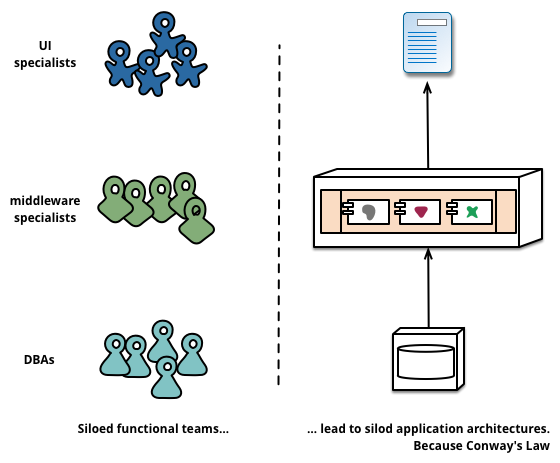
\includegraphics[width=\linewidth]{images/conways-law.png}
	\caption{Conway's Law in action \cite{ms-definition}}
	\label{fig:conway}
\end{figure}

In regards to MS, we divide the work force according to
\textit{business capabilities} rather than application layers. This
implies that our resulting team will be
cross-functional\footnote{meaning that our team is comprised of people
with different expertises, all working closely together for a common
goal}, combining the full range of skills required to develop the
service in question. This division leads us to Figure
\ref{fig:team-boundaries}.

% Before we move on, an interesting point to note here is the
% decreased
Here we see the decreased need for \textit{centralized management}
mentioned in the first simple definition presented above. To give an
example \cite{central-decentral}, centralized management is a
structure where only a few individuals make most of the decisions in a
company. We can find hierarchies within such a structure, each having
to respond to the superior's communicate. 

Decentralized management on the other hand would for example allow a
manager at a call center or retail store to make instant decisions
that impact their work environment. Thus, the decisions are not taken
solely by the higher ups but responsibilities are spread across
sectors—which could further spread responsibilities. This is an
interesting analogy to illustrate the new division of teams.

\begin{figure}
	\centering
	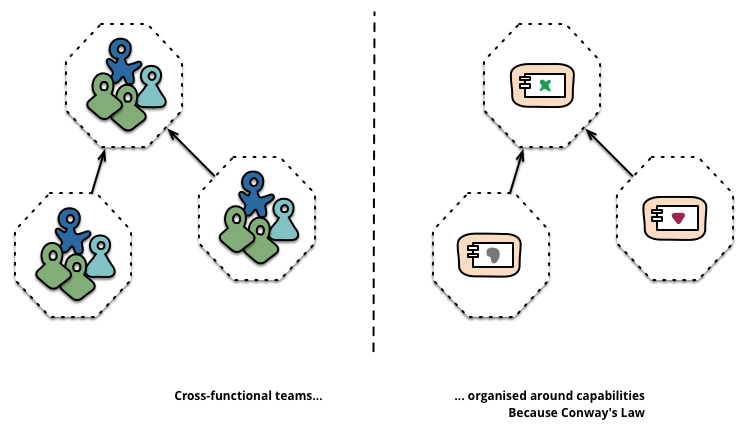
\includegraphics[width=\linewidth]{images/PreferFunctionalStaffOrganization.png}
	\caption{Service boundaries reinforced by team boundaries \cite{ms-definition}}
	\label{fig:team-boundaries}
\end{figure}

\subsubsection{Products not Projects}

Most of the application development focuses on delivering a piece of
software which is then considered completed. It is then handed over to
a separate maintenance team and the original team that built it will
then completely abandon the project. \cite{ms-definition}

The \gls{ms} philosophy tries to avoid this approach and instead
considers that a team should be responsible for its own product over
the full lifetime. Here is also a link to \textit{business
capabilities} in that software is no longer considered as a set of
functionalities that need to be completed. Rather it is seen as an
on-going relationship where one strives to enhance the business
capabilities.  \cite{ms-definition}

% \subsubsection{Smart endpoints and dumb pipes}

% Often times when it comes to process communication, great importance
% is put on the communication mechanism itself. With regards to
% microservices however, we place greater importance on the endpoints
% rather than the pipes. \cite{ms-definition}

% Thus one should strive to decouple the \glspl{ms} and keep them as
% cohesive as possible. In a way, they follow the Unix
% philosophy in that they receive a request, treat it appropriately, and
% then return a response. \gls{ms} can achieve this by using simple
% REST-like protocols. \cite{ms-definition}

% This further highlights that services in a microservice architecture
% are to be isolated components. When they communicate, the
% magic happens on the services' endpoints and not in the message
% bus---in fact we need nothing more for messages than simply being
% transferred from one endpoint to the other. \cite{ms-definition}

% \subsubsection{Decentralized Governance}

% Centralized governance that often comes along with monolithic
% architectures have the tendency to standardize on single technology
% platforms, which can be restricting. Rarely can a single language's
% full potential be leveraged for the entirety of an application.
% \cite{ms-definition}

% Splitting our application into services however, we do have the
% ability and choice of building each service with whatever tool is best
% for the job.

% This approach also brings a different mindset into development.
% Instead of focusing solely on the final product,
% developers prefer the idea of creating useful tools that can
% potentially also be used by other developers to solve similar
% problems. \cite{ms-definition}

\subsubsection{Decentralized Data Management} 
\label{sec:decentralized}

Monolithic applications usually prefer to have a single logical
database for persistent data, which in turn are then often used across
a range of applications. Microservices on the other hand let each
service manage its own data. Both situations are illustrated in 
figure \ref{fig:databases}. \cite{ms-definition}

The issue that arises with decentralizing the data, however, is
consistency.  Managing this is in fact not an easy task and usually
comes at the cost of increased computing times, leading to
\textit{eventual consistency}\footnote{When data is distributed, this
	refers to the assumption that we will eventually obtain the last
	updated value---since updates need to be propagated through each
	distributed system.} being solved through \textit{compensation
operations}\footnote{Referring to the fact that businesses are often
capable of handling a degree of inconsistency in favor of quick
responses to demands.} being the preferred method.
\cite{ms-definition}

\begin{figure}
	\centering
	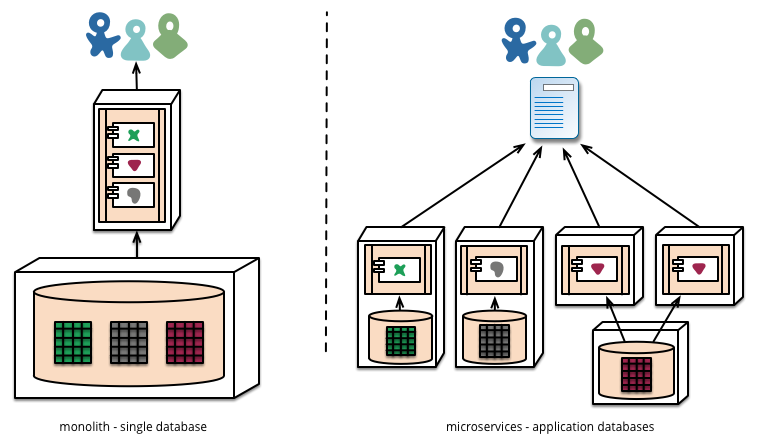
\includegraphics[width=\linewidth]{images/decentralised-data.png}
	\caption{Monolith and Microservice Databases \cite{ms-definition}}
	\label{fig:databases}
\end{figure}

\subsubsection{Infrastructure Automation}
\label{sec:infrastructure-automation}

Many products following the \gls{ms} architecture make heavy use of
\gls{cicd} and infrastructure automation tools. This becomes
especially relevant in production when you have to manage a lot of
different \glspl{ms} at once, which simply becomes infeasible without
the automation.  \cite{ms-definition}

\subsubsection{Design for failure}
\label{sec:design-for-failure}

One needs to take into consideration that a service may fail at any
point in time for whatever reason, and the client should respond to
this as gracefully as possible. Due to the decoupled nature of
\glspl{ms}, we have an additional complexity to take into account
which constantly requires us to reflect on how service failure can
affect the user experience. \cite{ms-definition} It should be noted
that service failure is different from a regular application failure.
For the latter, it will most likely cause the entire application to
break and terminate. A service failure will only break the service in
question, other services will not be terminated as a result but keep
running independently.

It is therefore of utmost importance to detect failures quickly and
restore the service. To achieve this, a lot of sophisticated
monitoring and logging on various parts of a service are
performed---with great focus on inter-service communication.
\cite{ms-definition}


\subsection{Assessment}% (± 15\% of section's words)}
% {\color{gray}
% Provide any objective elements to assess that your deliverables do or do not satisfy the requirements described above. 
% }

Given all the above, there are drawbacks that come with the
microservice architecture. As pointed out in
section \nameref{sec:design-for-failure}, a service can fail at any point
in time which makes it quite difficult to build distributed systems.
Added to this, remote call are slow which can also have an impact of
the final product's performance. Another drawback that we discussed
in section \nameref{sec:decentralized} is the issue of eventual
consistency.

As slightly touched upon in the
\nameref{sec:infrastructure-automation} section, we will run into the
issue of \textit{operational complexity}\footnote{While small
	independent services are easy to deploy, the number of services adds
strain to the complexity regarding operations}, demanding a mature
operations team plus a performant software environment meant to
support their daily activities.
% to manage lots of services, which are being redeployed
% regularly.
A product consisting of half-a-dozen applications can
quickly expand into hundreds of little microservices.
\cite{ms-trade-off}

% We can see that working with \glspl{ms} is not a simple task.
% \cite{ms-arch-study} There are in fact many more aspects stemming from
% \glspl{ms} that cause complications in the development of such systems
% \cite{ms-pains-gains} which we shall not dive into in this report.

For these reasons, the role of DevOps comes into play to ease this whole process.
It becomes increasingly harder, tedious and eventually impossible to
manage an increasing number of services which will call for a lot of
automation and monitoring to take place. Nonetheless, given that \glspl{ms} are
smaller and thus easier to understand, problems are likely to occur in
the interconnections of such services which potentially makes it very
difficult to trace and debug issues---hence the need for proper and
elaborate monitoring.


% \KB{Highlight elements pointing to TD?}
